\documentclass[11pt]{article}
\usepackage[a4paper,margin=2.4cm]{geometry}
\usepackage[T1]{fontenc}
\usepackage{lmodern}
\usepackage{microtype}
\usepackage{amsmath,amssymb}
\usepackage{booktabs}
\usepackage{graphicx}
\usepackage{caption}
\usepackage{setspace}
\usepackage{enumitem}
\usepackage{xcolor}
\usepackage[authoryear,round]{natbib}
\usepackage[colorlinks=true,linkcolor=black,citecolor=blue!60!black,urlcolor=blue!60!black]{hyperref}
\captionsetup{font=small,labelfont=bf,skip=4pt}
\setlist{nosep,leftmargin=1.4em,topsep=2pt}
\setstretch{1.12}
\graphicspath{{../output/figures/}}
\newcommand{\tabpath}{../output/tables}
\input{\tabpath/macros_desc.tex}
\input{\tabpath/macros_sel.tex}
\input{\tabpath/macros_bench.tex}
\input{\tabpath/macros_main.tex}
\input{\tabpath/macros_vol.tex}
\input{\tabpath/macros_rob.tex}
\newcommand{\SUEA}{SUE^{A}}
\newcommand{\SUEQ}{SUE^{Q}}
\newcommand{\note}[1]{\par\vspace{2pt}{\footnotesize\setstretch{1.0}\leftskip=0pt\rightskip=0pt%
\parfillskip=0pt plus 1fil\noindent #1\par}}

\title{\textbf{Two Reports, One Day:\\ Do Investors Neglect Bundled Earnings News?}}
\author{}
\date{Draft, October 2026}

\begin{document}
\maketitle
\vspace{-2em}
\begin{abstract}
\noindent Chinese listed firms must publish their annual report and their first-quarter (Q1) report by 30 April, and
the Q1 report may not appear before the annual report. As annual reports drifted toward the deadline, the share of
firms that release both reports on the same day rose from \ShareSDearly\% to \ShareSDlate\% between 2006 and 2020.
Such bundles give a clean, within-firm test of limited attention: two earnings signals of the same kind arrive at
once. A naive comparison suggests that investors neglect the older signal. The stock-price response to the annual
earnings surprise is \NaiveDropPct\% lower when the Q1 report arrives in the same month. We show that this gap is an
artefact of comparing different information sets. Once both reports are public for every firm, the response to the
annual surprise is the same. Comparing firms that filed their annual report on the same day, and letting each filing
date have its own earnings response, bundling changes neither the price response to either surprise nor the later
drift. Trading volume reacts, if anything, more strongly to bundled news. Bundling is mostly a mechanical by-product
of late annual reporting, and firms do not use it to bury bad annual news. Muted reactions to bundled disclosures
should not be read as inattention without aligning what investors know.

\medskip\noindent\textbf{Keywords:} limited attention, disclosure bundling, earnings announcements, information
overload, China.\quad \textbf{JEL:} G14, G41, M41.
\end{abstract}

\section{Introduction}

Attention is scarce. Investors cannot read everything at once, and a large literature argues that this limits how
quickly prices absorb public information \citep{kahneman1973,sims2003,hirshleifer2003,peng2006,blankespoor2020}. If
attention is scarce, then \emph{how} a firm packages its news should matter. Two pieces of news released together
compete for the same few hours of investor attention; released a week apart, each gets its own. This concern is
behind evidence that concurrent releases of earnings and the 10-K receive muted reactions and more drift
\citep{arif2019}, that managers spread disclosures out to avoid overload \citep{chapman2019}, and that managers bundle
or time bad news when attention is low \citep{dehaan2015,segal2016,michaely2016}.

Testing whether packaging \emph{causes} neglect is hard. Firms choose their packages. The pieces of a typical bundle,
such as an earnings release with a management forecast, are different kinds of news, which makes it difficult to
measure the surprise in each \citep{rogers2013}. And the reactions of bundled and unbundled news are compared at
moments when investors know different things.

We study a setting that removes most of these problems. In China, two rules create bundles. Both the annual report
and the Q1 report are due by 30 April, and the Q1 report may not be published before the annual report
\citep{csrc_disclosure,sse_rules}. A firm that files its annual report on 26 April must therefore publish its Q1
report between 26 and 30 April, often on the same day (Figure~\ref{fig:timeline}). As annual reports moved toward
the deadline, same-day bundles rose from \ShareSDearly\% of firm-years in 2006--2011 to \ShareSDlate\% in 2020. Each
bundle contains two earnings numbers of the same kind, the fourth-quarter result inside the annual report and the
next Q1 result, which we measure with the same expectation model.

A naive look at the data suggests textbook neglect. In the month of the annual report, the stock-price response to
the annual earnings surprise is \NaiveSep\% per unit of surprise when the Q1 report comes in a later month, but only
\NaiveSD\% when both reports come out on the same day: a \NaiveDropPct\% drop ($t=\NaiveSDdiffT$). We argue that
this comparison is wrong, for two reasons, and design the tests around them.

The first reason is \emph{information sets}. When the Q1 report comes a month later, investors price the annual
surprise without knowing Q1. A good annual result predicts a good Q1, so part of the price response to the annual
surprise is really a forecast of Q1. When both reports arrive together, that forecast is replaced by the actual Q1
number, and the price response is rightly attributed to the Q1 surprise. An efficient market therefore reacts less
to a bundled annual surprise, without any inattention. Once we compare returns over a window in which both reports
are public for every firm, the gap disappears: \AlignedSep\% versus \AlignedSD\% ($t=\AlignedSDdiffT$).

The second reason is \emph{selection}. Bundlers are late filers with worse news. Our main design therefore compares a
bundling firm only with firms that filed their annual report \emph{on the same day} but published Q1 a few days later
in the same month. By the end of that month the two groups have released exactly the same kind of information. We let
each filing date have its own response to both surprises, so that any news, crowding or lateness that is common to the
date cancels out. In other specifications we let each firm have its own response, comparing the same firm in years it
bundles with years it does not. Across these designs bundling has no effect on the price response to either surprise,
and no effect on the drift over the next three months. For the Q1 surprise we can rule out that bundling lowers the
response by more than \MainRuleOutQ\% of its normal size. Trading volume, an independent measure of attention, does
not respond less to bundled news; it responds more to the size of a bundled Q1 surprise ($t=\VolQtwoT$).

Who bundles, and why? The lateness of the annual report explains most of it: each decile of lateness raises the
probability of a same-day release by \SelLate{} percentage points. Holding the filing date fixed, firms with bad
annual news are not more likely to bundle, so bundling is not used to bury bad annual news, and bundled bad news is not
priced less. Firms with bad Q1 news are \emph{less} likely to bundle, consistent with the older finding that bad news
is delayed \citep{givoly1982,haw2000}.

The paper makes three contributions. First, it provides clean evidence that releasing two earnings signals on the
same day does not cause investors to neglect either of them, at least at a monthly horizon. This complements the
evidence that macro news makes investors process firm news \emph{better} \citep{hirshleifer2022}, and the finding of
\citet{segal2016} that strategically bundled news shows no sign of investor inattention. It qualifies the
interpretation of muted reactions to concurrent releases \citep{arif2019}. Second, it shows a simple bias in such
comparisons and a simple fix: whenever one signal in a package predicts the other, compare responses over a window in
which both are public. Third, it documents China's April reporting crunch and shows how a sequencing rule turns late
reporting into bundling, which adds to work on the timing of Chinese annual reports
\citep{haw2000,you2011,li2020}.

\begin{figure}[t]
\centering
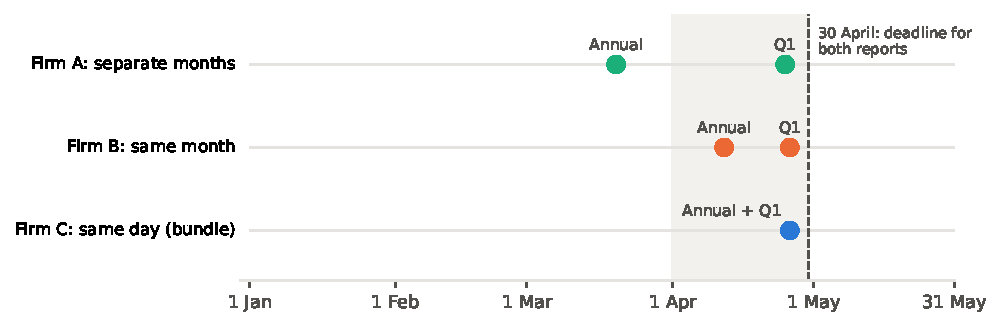
\includegraphics[width=0.9\textwidth]{fig_timeline.pdf}
\caption{Three ways to publish the annual and the Q1 report. Both reports are due by 30 April, and the Q1 report may
not come first. Firm A files its annual report in March and its Q1 report in late April (separate months). Firm B
files both in April, a few days apart (same month). Firm C files both on the same day (a bundle). By the end of
April all three firms have published the same two reports.}
\label{fig:timeline}
\end{figure}

\section{Institutional setting and hypotheses}

\paragraph{Reporting rules.} Chinese A-share firms must publish the annual report within four months of the fiscal
year end (31 December), that is, by 30 April, and the Q1 report within one month of the quarter end, also by 30
April. The Q1 report may not be disclosed before the previous year's annual report \citep{csrc_disclosure,sse_rules}.
The exchanges schedule disclosure dates in advance, and many firms crowd into the last week of April. Annual reports
give the full-year figures, so the new earnings information they contain beyond the three earlier quarterly reports
is the fourth-quarter result. We call the surprise in it the \emph{annual surprise}, $\SUEA$. The Q1 report gives the
first quarter of the new year; we call its surprise the \emph{Q1 surprise}, $\SUEQ$.

\paragraph{Hypotheses.} If attention is limited, a bundle should get less of it per signal
\citep{hirshleifer2003,hirshleifer2009}:

\begin{itemize}
\item \textbf{H1 (neglect).} When the two reports are released together, the price reacts less to at least one of the
surprises in the release month, more of the reaction comes later (drift), and trading volume responds less.
\item \textbf{H0 (full processing).} Given the same information and timing, the package does not matter.
\item \textbf{H2 (burying).} Managers bundle bad annual news to soften its price impact
\citep{dehaan2015,segal2016,li2020}.
\end{itemize}

H1 does not say \emph{which} signal is neglected. The annual report is the more salient document. It is long, audited
and comes with dividends and a full-year headline \citep{huang2018}. The Q1 number is the more recent and, for
forecasting, more relevant one; people tend to weight the most recent evidence more \citep{hogarth1992}, and older
information moves prices less \citep{tetlock2011}. Our tests are symmetric and allow either signal to be neglected.

\section{Data}

\paragraph{Sample.} We use monthly data on all stocks traded on the Shanghai and Shenzhen exchanges from Thomson
Reuters Datastream and Worldscope, including inactive stocks to avoid survival bias \citep{shumway1997}. The panel
gives prices, total return indices, trading volume, shares outstanding, book values and standalone quarterly
earnings per share (EPS) together with each report's publication date. We pair every annual report for fiscal year
$Y$ with the Q1 report of $Y+1$, for $Y=2005$ to $2019$ (reports published in 2006--2020). Table~\ref{tab:sample}
shows how the sample of \NFirmYears{} firm-years from \NFirms{} firms is built. We classify each firm-year by the
timing of the two reports: \emph{same day} (\NSameDay), \emph{same month} (\NSameMonth; median gap \MedianGapSM{}
days) and \emph{separate months} (\NSeparate). Publication dates in Datastream can differ from the official filing
by a day, because many reports are filed in the evening or at weekends. Spot checks against the filings confirm the
classification. Hikvision published its 2017 annual report and 2018 Q1 report together on 21 April 2018, and
Industrial Bank presented its 2018 annual and 2019 Q1 results together on 29 April 2019. A one-day error does not
affect our monthly tests unless it moves a report across a month boundary, a case our robustness tests cover.

\paragraph{Measuring news.} We measure each surprise against a seasonal random walk (SRW): expected EPS equals EPS of
the same quarter a year earlier \citep{foster1977,bernard1990}. The surprise is scaled by the standard deviation of the
firm's last eight SRW errors. For example, if Q1 EPS is 0.30 against 0.25 a year earlier and past errors have a
standard deviation of 0.05, then $\SUEQ=(0.30-0.25)/0.05=1$. The SRW has a key advantage here: its expectation does
not depend on the order of the releases. A statistical forecast made just before a bundled release cannot use the
fourth-quarter number, but one made before a separate Q1 release can. That would make Q1 surprises incomparable
across groups. We use an out-of-sample XGBoost forecast \citep{chen2016} as a robustness check.

\paragraph{Returns and volume.} Returns are monthly and size-adjusted: each stock's return minus the average return of
its size decile in that month. A report published on 26 April therefore shows up in the April return. This sounds
crude, but it matters less than it seems: by the end of April, firms that bundled and firms that published the two
reports a few days apart have revealed exactly the same information, so their April returns can be compared directly.
Abnormal turnover is the log of monthly turnover minus the firm's average over the preceding year.

\paragraph{Descriptive statistics.} Figure~\ref{fig:trends} shows the rise of bundling. Until 2012 fewer than 6\% of
firm-years were same-day bundles; by 2020 nearly half were (panel a). The rise mirrors a shift of annual reports
toward the deadline: the median report came \LagEarly{} days after the year end until 2015 and \LagLate{} days in 2020
(panel b). Bundling is almost entirely a late-filer phenomenon: \ShareSDbottomHalf\% of firms in the earlier half of
each year's filing order bundle, against \ShareSDtopLate\% of the latest fifth (panel c). Table~\ref{tab:desc} shows
that bundlers file their annual report \(116\) days after the year end, against 83 days for firms that publish in
separate months. They also bring worse annual news (mean $\SUEA$ of $-0.76$ against $0.28$) and more losses (18\%
against 8\%). They are similar in size and analyst coverage. Selection on news is therefore a first-order concern.

\begin{table}[t]
\centering
\begin{minipage}[t]{0.40\textwidth}
\captionof{table}{Sample construction}\label{tab:sample}
\centering\footnotesize
\input{\tabpath/tab_sample_flow.tex}
\note{Firm-years pair the annual report for fiscal year $Y$ with the Q1 report of $Y+1$.}
\end{minipage}\hfill
\begin{minipage}[t]{0.57\textwidth}
\captionof{table}{Descriptive statistics by release pattern}\label{tab:desc}
\centering\footnotesize
\resizebox{\linewidth}{!}{\input{\tabpath/tab_descriptives.tex}}
\note{Means. Surprises are SRW-based and scaled by the SD of the firm's past errors. Abnormal turnover is log
turnover minus the firm's average over months $-12$ to $-2$.}
\end{minipage}
\end{table}

\begin{figure}[t]
\centering
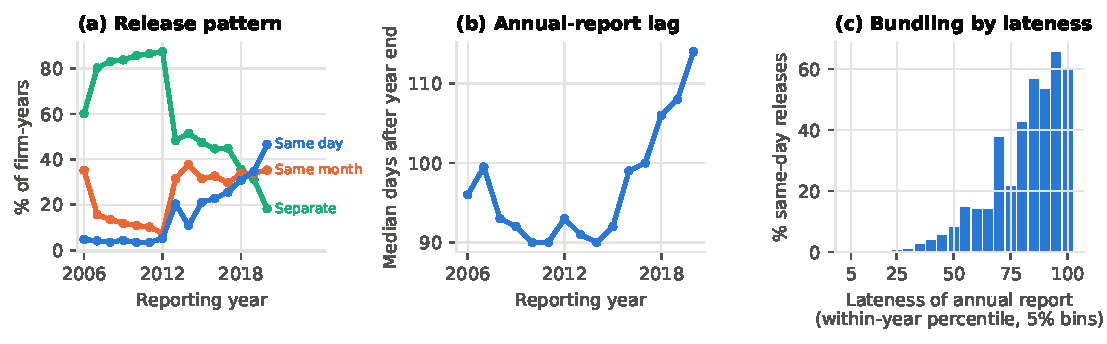
\includegraphics[width=\textwidth]{fig_bundling_trends.pdf}
\caption{The rise of bundling. (a) Share of firm-years by release pattern. (b) Median number of days between the
fiscal year end and the annual report. (c) Share of same-day releases by the lateness of the annual report within
its year (percentile of the filing order).}
\label{fig:trends}
\end{figure}

\section{Methodology}

\paragraph{The naive test.} The obvious test regresses the return in the month of the annual report on the annual
surprise and lets the slope differ by release pattern:
\begin{equation}
\begin{split}
R_{i,m} = \alpha_m &+ \beta\,\SUEA_i + \gamma_{SM}\,\SUEA_i\times SM_i + \gamma_{SD}\,\SUEA_i\times SD_i\\
&+ \theta\,\SUEQ_i\times(SM_i+SD_i) + \text{dummies} + \varepsilon_i ,
\end{split}
\label{eq:naive}
\end{equation}
where $SM$ and $SD$ mark same-month and same-day releases, $\alpha_m$ are month fixed effects, and the $\SUEQ$ term
captures the Q1 news in months that contain both reports. H1 predicts $\gamma_{SD}<0$.

\paragraph{Why the naive test is biased: information sets.} Suppose the market is efficient and a one-unit annual
surprise predicts a Q1 surprise of $\rho$ units. A firm that reports in separate months first earns $\beta\,\SUEA$
in the annual-report month, where $\beta$ includes the expected Q1 news. When Q1 arrives, the firm earns
$\beta_Q(\SUEQ-\rho\,\SUEA)$, the part of Q1 that was not expected. Adding the two months, the total response to the
annual surprise is $\beta-\beta_Q\rho$. A bundling firm reveals both numbers at once, so its single month carries
exactly this total: $(\beta-\beta_Q\rho)\SUEA+\beta_Q\SUEQ$. Even an efficient market thus reacts \emph{less} to a
bundled annual surprise, by $\beta_Q\rho$. In words, when a strong annual result comes alone, investors also price
the strong Q1 they now expect. When the actual Q1 number arrives at the same time, that part of the price move is
credited to Q1. The fix is to compare returns over a window in which both reports are public for every firm: from the
annual-report month to the Q1-report month.

\paragraph{Main design: same filing date.} To deal with selection we compare each bundling firm only with firms that
published their annual report on the same day but their Q1 report a few days later in the same month. Within the
firm-years whose two reports fall in the same month, we estimate
\begin{equation}
R_{i,m} = \alpha_d + \beta_d\,\SUEA_i + \kappa_d\,\SUEQ_i + \lambda\, B_i + \delta_A\, B_i\times\SUEA_i
+ \delta_Q\, B_i\times\SUEQ_i + \varepsilon_i ,
\label{eq:main}
\end{equation}
where $B_i$ marks a bundle and $d$ is the annual-report date. Every date has its own intercept \emph{and} its own
response to both surprises ($\beta_d,\kappa_d$). For example, on a given day in late April a few dozen firms publish
annual reports; some publish Q1 the same day and the rest a few days later. Equation~\eqref{eq:main} compares only
these firms with each other. Anything that is common to the date drops out: market-wide news, the number of other
firms reporting that day \citep{hirshleifer2009,you2011}, and how late the date is. H1 predicts $\delta_A<0$ or
$\delta_Q<0$ in the release month, and the opposite sign in later months. In further specifications each firm has
its own intercept and slopes, so the comparison is between years in which the \emph{same} firm bundles and years in
which it does not \citep[ch.~8]{cunningham2021}. We estimate the models by partialling out the group-specific
intercepts and slopes (the Frisch--Waugh--Lovell theorem, \citealp{lovell1963}). Standard errors are clustered by
filing date and by firm \citep{petersen2009,cameron2011}.

\paragraph{Volume.} Prices can be slow even when investors pay attention, and attention can rise without moving
prices. We therefore also replace the return with abnormal turnover and the surprises with their absolute values. H1
predicts that turnover responds less to the size of bundled news.

\section{Results}

\subsection{Who bundles?}

Table~\ref{tab:sel} estimates linear probability models of a same-day release. Lateness dominates. Each decile of
the filing order raises the probability of a bundle by \SelLate{} percentage points (column 1), against a base rate of
\SelBaseRate\%. Without controlling for the filing date, bad annual news predicts bundling (\SelNegAyear{} points,
$t=\SelNegAyearT$). Once firms are compared with others that filed on the same day (column 3), bad annual news no
longer matters (\SelNegAdate{} points, $t=\SelNegAdateT$). Bad annual news predicts bundling only because it predicts
late filing \citep{givoly1982,haw2000}. Bad Q1 news, in contrast, makes a bundle \emph{less} likely: it changes the
probability by \SelNegQdate{} points ($t=\SelNegQdateT$), also within firm (column 4). Figure~\ref{fig:sel} shows the same pattern
without regression assumptions: given the filing date, the probability of a bundle is flat in the annual surprise but
rises with the Q1 surprise from the fourth decile upward (only the very worst decile breaks the pattern). Firms that file the annual report late and have good Q1 news publish both together; those
with bad Q1 news take the remaining days. This fits delaying bad news, not burying bad annual news.

\begin{table}[t]
\begin{minipage}[t]{0.60\textwidth}
\captionof{table}{Who bundles?}\label{tab:sel}
\centering\footnotesize
\resizebox{\linewidth}{!}{\input{\tabpath/tab_selection.tex}}
\note{Linear probability models of a same-day release, in percentage points. $t$-statistics in parentheses,
clustered by firm (columns 1--2) and by firm and annual-report date (3--4). *, **, ***: 10\%, 5\%, 1\%.}
\end{minipage}\hfill
\begin{minipage}[t]{0.37\textwidth}
\captionof{figure}{Bundling and news, same filing date}\label{fig:sel}
\centering
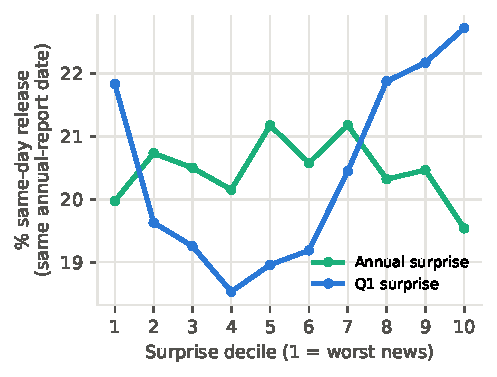
\includegraphics[width=\linewidth]{fig_selection.pdf}
\note{Share of same-day releases by surprise decile, after removing annual-report-date effects.}
\end{minipage}
\end{table}

\subsection{The naive gap and the information-set benchmark}

Table~\ref{tab:bench} column 1 reproduces the naive result. The response to the annual surprise in its release month
falls from \NaiveSep\% for firms that publish in separate months to \NaiveSM\% (same month) and \NaiveSD\% (same day).
Columns 2--4 trace the information-set argument. For separate-month firms the annual surprise earns \NaiveSep\% in
its own month (column 2). When Q1 arrives, part of that response is reversed. The annual surprise loads at
\BenchCorrection\% on the Q1-month return, given the Q1 surprise ($t=\BenchCorrectionT$; column 3). The net response
once both reports are public is about \BenchPredPath\%, close to what the simple rule predicts with $\rho=\BenchRho$
and $\beta_Q=\BenchQoneSep$ (\BenchPredRho\%). This is already much closer to the bundled firms' \BenchJoint\%
(column 4). The rest of the difference comes from measuring the two groups over different windows. Column 5 makes the comparison directly, over the window from the
annual-report month to the Q1-report month. The annual-surprise slopes are now the same: the bundle interaction is
zero ($t=\AlignedSDdiffT$). Figure~\ref{fig:aligned} shows the two comparisons side by side.

Column 5 also shows a lower Q1-surprise slope for bundled and same-month firms ($t=\AlignedQoneSDT$). This is not
evidence of neglect. Separate-month firms have longer windows that start earlier and also absorb information about Q1
before the Q1 report. They are also early filers, a different kind of firm. The same-date design below removes both
differences.

\begin{table}[t]
\captionof{table}{The naive comparison and the information-set benchmark}\label{tab:bench}
\centering\footnotesize
\resizebox{\linewidth}{!}{\input{\tabpath/tab_naive_benchmark.tex}}
\note{Size-adjusted returns in \% per unit of surprise. Column 1 uses all firm-years and the annual-report month.
Columns 2--3 use separate-month firms and the annual-report and Q1-report months. Column 4 uses firms whose two
reports fall in the same month. Column 5 uses the window from the annual-report month to the Q1-report month. Fixed
effects for the calendar month in which the window starts (1--2, 4) or ends (3, 5). $t$-statistics clustered by
month and firm.}
\end{table}

\begin{figure}[t]
\centering
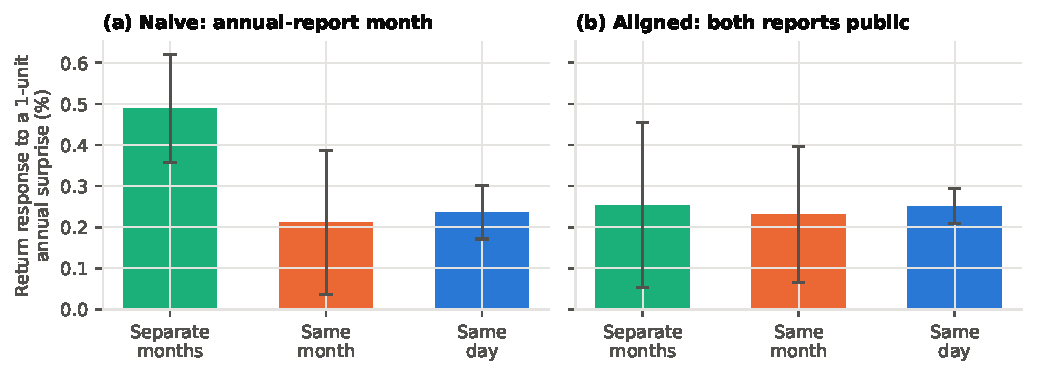
\includegraphics[width=0.92\textwidth]{fig_naive_vs_aligned.pdf}
\caption{Response to the annual surprise by release pattern. (a) Return in the annual-report month only. (b) Return
over the window in which both reports are public. Bars show the slope on $\SUEA$ (\% per unit); lines show 95\%
confidence intervals.}
\label{fig:aligned}
\end{figure}

\subsection{Main result: bundles versus firms filing on the same date}

Table~\ref{tab:main} reports Equation~\eqref{eq:main} for the \MainN{} firm-years whose two reports fall in the same
month, filed on \MainNdates{} annual-report dates. With date effects only (column 1), the normal release-month
responses are \MainBaseA\% for the annual and \MainBaseQ\% for the Q1 surprise. Bundling changes neither: the
interactions are \MainAoneD{} ($t=\MainAoneT$) and \MainQoneD{} ($t=\MainQoneT$). Letting every date have its own
response (column 2), every firm have its own response (column 3) or both (column 4) leaves the interactions small and
insignificant. Extending the window by one month (column 5), which captures reports filed in the evening of the last
days of April, gives two estimates of opposite sign near the 5\% level, a pattern we discuss below. The drift over the next
three months (column 6) shows no delayed reaction to either bundled surprise. Bundled firms do earn
\MainBundleLevelPost\% more over these three months whatever their news ($t=\MainBundleLevelPostT$). This is a level
difference between kinds of late filers, not a delayed response to the surprises, and we leave it for future work.

How large an effect can we exclude? In column 2 the 95\% confidence interval for the bundle effect on the Q1 response
is [\MainCIQlo, \MainCIQhi], so a reduction of more than \MainRuleOutQ\% of the normal Q1 response is ruled out. The
annual surprise moves prices little in its release month to begin with (\MainBaseA\%), so its interval
[\MainCIAlo, \MainCIAhi] is less informative on its own.

Figure~\ref{fig:paths} adds the time dimension. It plots the cumulative response to each surprise from January, for
bundled and same-month firms filing on the same date. The Q1 paths lie on top of each other before, during and after
the release month. The annual-surprise paths differ slightly, but the gap opens in \emph{March}, before either report
is out, and stays constant afterwards. That is a difference between the kinds of firms, not an effect of the bundle.
The column 5 estimates are not robust. They appear only with date-specific slopes, and in Figure~\ref{fig:paths} the
April--May increments of the two groups are almost identical. Neither the release month nor the next three months
shows them. With twelve bundle coefficients in Table~\ref{tab:main}, one estimate at the 5\% level is about what
chance alone would produce.

\begin{table}[t]
\captionof{table}{Main result: bundled versus same-month firms with the same annual-report date}\label{tab:main}
\centering\footnotesize
\input{\tabpath/tab_same_date.tex}
\vspace{4pt}
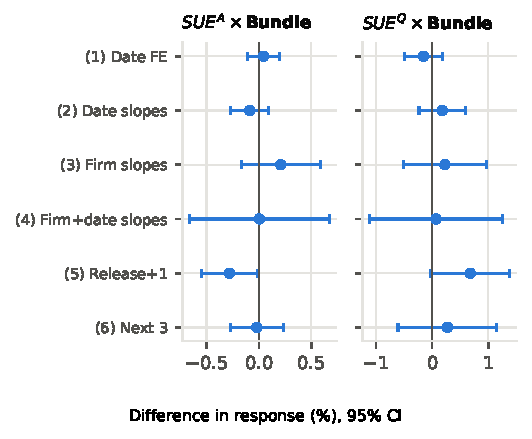
\includegraphics[width=0.52\textwidth]{fig_coefplot.pdf}
\note{Sample: firm-years whose annual and Q1 reports fall in the same calendar month. Bundle = both on the same day.
Dependent variable: size-adjusted return (\%) in the release month (1--4), the release and the next month (5), or the
three following months (6). Date-specific slopes let each annual-report date have its own response to $\SUEA$ and
$\SUEQ$; firm-specific slopes do the same for each firm. $t$-statistics two-way clustered by date and firm. The plot
shows the bundle interactions with 95\% confidence intervals.}
\end{table}

\begin{figure}[t]
\centering
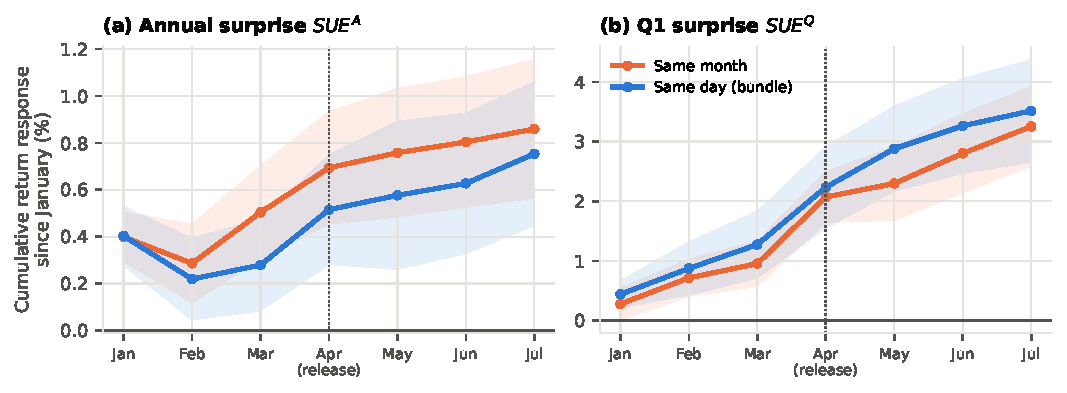
\includegraphics[width=0.95\textwidth]{fig_event_paths.pdf}
\caption{Cumulative response to the two surprises, bundled versus same-month firms. Each point is the slope of the
cumulative size-adjusted return from January to the given month on the surprise, from a regression with annual-report
date effects. Bands are 95\% confidence intervals. Month 0 is the release month (April for 97\% of the sample).}
\label{fig:paths}
\end{figure}

\subsection{Trading volume}

If a bundle diverted attention, fewer investors would trade on its content. Table~\ref{tab:vol} shows the opposite.
Within a filing date, turnover in bundled firms responds \emph{more} to the size of the Q1 surprise
(\VolQtwo{} percentage points per unit of $|\SUEQ|$, $t=\VolQtwoT$), and no differently to the size of the annual
surprise. The result weakens when each firm gets its own slope (column 4). Figure~\ref{fig:vol} shows the raw
pattern. Bundles look like days of concentrated rather than divided attention, in line with the complementarity of
news found by \citet{hirshleifer2022}.

\begin{table}[t]
\begin{minipage}[t]{0.58\textwidth}
\captionof{table}{Trading volume}\label{tab:vol}
\centering\footnotesize
\resizebox{\linewidth}{!}{\input{\tabpath/tab_volume.tex}}
\note{Dependent variable: abnormal turnover in the release month (\%). Same sample as Table~\ref{tab:main}.
$t$-statistics two-way clustered by date and firm.}
\end{minipage}\hfill
\begin{minipage}[t]{0.39\textwidth}
\captionof{figure}{Turnover and surprise size}\label{fig:vol}
\centering
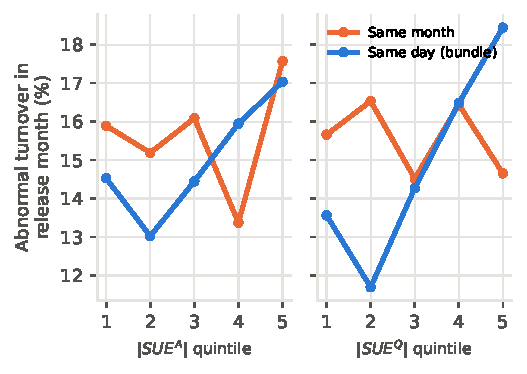
\includegraphics[width=\linewidth]{fig_volume.pdf}
\note{Abnormal turnover by quintile of the absolute surprise, after removing date effects.}
\end{minipage}
\end{table}

\subsection{Heterogeneity, robustness, burying and a placebo}

Table~\ref{tab:rob} repeats the main specification (column 2 of Table~\ref{tab:main}) in subsamples and variations.
If attention constraints mattered anywhere, they should matter for small firms and firms without analyst coverage,
where fewer investors watch. Neither shows a significant Q1 effect. Small firms show a borderline annual effect
(\RobSmallA, $t=\RobSmallAT$), but no Q1 effect, and the annual effect does not reappear in any other subsample. The results hold before and after 2012, without the
2020 reporting season, when COVID-19 delayed many reports, without loss firms, with XGBoost annual surprises, and over
a two-month window. Across \RobNtests{} rows and two coefficients each, \RobNsig{} rows contain an estimate at the 5\% level, close to
the 1.2 that chance alone would produce.

We test burying directly by letting the bundle effect differ for bad annual news. A bundle does not soften the
response to bad annual news in the release month (\BuryRel, $t=\BuryRelT$) or over January--July (\BuryJJ,
$t=\BuryJJT$). Finally, a placebo assigns ``treatment'' to same-month firms that will bundle \emph{next} year. If our
estimates captured persistent firm types rather than bundling, the placebo would show the same pattern. It does not
(\RobPlaceboQ, $t=\RobPlaceboQT$).

\begin{table}[t]
\begin{minipage}[t]{0.60\textwidth}
\captionof{table}{Heterogeneity, robustness, burying and placebo}\label{tab:rob}
\centering\footnotesize
\resizebox{\linewidth}{!}{\input{\tabpath/tab_robustness.tex}}
\note{Each row re-estimates column 2 of Table~\ref{tab:main}. Coefficients in \% ($t$-statistics). Small and large
firms split at the yearly median of size. The placebo uses same-month firms only and marks those that bundle in the
following year. The burying rows add $\SUEA\times$Bundle$\times$(bad annual news) with date-specific slopes.}
\end{minipage}\hfill
\begin{minipage}[t]{0.37\textwidth}
\captionof{figure}{Bundle effects across tests}\label{fig:forest}
\centering
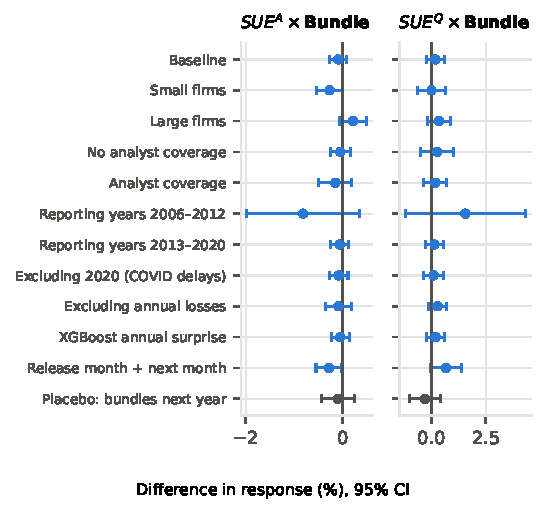
\includegraphics[width=\linewidth]{fig_forest.pdf}
\note{Point estimates and 95\% confidence intervals from Table~\ref{tab:rob}; the placebo is grey.}
\end{minipage}
\end{table}

\section{Discussion}

Why do bundles not cause neglect? Three features of the setting help. First, a bundle concentrates attention as well
as news: the firm's reporting day attracts media coverage, analyst notes and trading, so the second document gets
read along with the first. Second, the Q1 report is short and its key number is easy to find, so the processing cost
of the second signal is low \citep{blankespoor2020}. Third, the information that matters for prices is set by the
marginal investor, who need not be the distracted one.

Our evidence has limits. Monthly returns cannot detect delays of a few days. \citet{fedyk2024} finds that the
response to less prominently placed news converges within about two days, which is well inside a month. What we can
say is that bundling does not leave news unpriced at the end of the release month or later. Publication dates come
from Datastream and can be off by a day. We do not observe Q1 preannouncements, which may tell investors part of the
Q1 news before the report; such leaks would affect bundled and same-month firms filing on the same date alike.
Finally, the same-date design compares firms that filed the annual report on the same day, and how firms choose
their filing date may still be correlated with news. The placebo and the firm-specific slopes address persistent
differences, but not time-varying ones.

\section{Conclusion}

China's reporting rules turned late annual reporting into a natural laboratory for bundled disclosure. A naive
comparison suggests that investors largely ignore the annual earnings surprise when the Q1 report arrives with it.
The gap disappears once investors' information sets are aligned. In comparisons among firms filing on the same day,
bundling changes neither the price response nor the later drift for either signal, and volume reacts more, not less.
Firms bundle because they file late, not to bury bad annual news. The broader lesson is methodological: when one
signal in a package predicts another, a muted reaction to that signal is what an efficient market should deliver,
and only a comparison over an aligned information window can tell neglect from rational updating.

\setstretch{1.0}
\small
\begin{thebibliography}{99}
\bibitem[Arif et~al.(2019)]{arif2019} Arif, S., Marshall, N.~T., Schroeder, J.~H., Yohn, T.~L., 2019. A growing
disparity in earnings disclosure mechanisms: The rise of concurrently released earnings announcements and 10-Ks.
\emph{Journal of Accounting and Economics} 68(1), 101221.
\bibitem[Bernard and Thomas(1990)]{bernard1990} Bernard, V.~L., Thomas, J.~K., 1990. Evidence that stock prices do not
fully reflect the implications of current earnings for future earnings. \emph{Journal of Accounting and Economics}
13(4), 305--340.
\bibitem[Blankespoor et~al.(2020)]{blankespoor2020} Blankespoor, E., deHaan, E., Marinovic, I., 2020. Disclosure
processing costs, investors' information choice, and equity market outcomes: A review. \emph{Journal of Accounting and
Economics} 70(2--3), 101344.
\bibitem[Cameron et~al.(2011)]{cameron2011} Cameron, A.~C., Gelbach, J.~B., Miller, D.~L., 2011. Robust inference with
multiway clustering. \emph{Journal of Business \& Economic Statistics} 29(2), 238--249.
\bibitem[Chapman et~al.(2019)]{chapman2019} Chapman, K., Reiter, N., White, H.~D., Williams, C.~D., 2019. Information
overload and disclosure smoothing. \emph{Review of Accounting Studies} 24(4), 1486--1522.
\bibitem[Chen and Guestrin(2016)]{chen2016} Chen, T., Guestrin, C., 2016. XGBoost: A scalable tree boosting system.
\emph{Proceedings of the 22nd ACM SIGKDD Conference}, 785--794.
\bibitem[CSRC(2021)]{csrc_disclosure} China Securities Regulatory Commission, 2021. Measures for the Administration of
Information Disclosure by Listed Companies. Beijing.
\bibitem[Cunningham(2021)]{cunningham2021} Cunningham, S., 2021. \emph{Causal Inference: The Mixtape}. Yale University
Press, New Haven.
\bibitem[deHaan et~al.(2015)]{dehaan2015} deHaan, E., Shevlin, T., Thornock, J., 2015. Market (in)attention and the
strategic scheduling and timing of earnings announcements. \emph{Journal of Accounting and Economics} 60(1), 36--55.
\bibitem[Fedyk(2024)]{fedyk2024} Fedyk, A., 2024. Front-page news: The effect of news positioning on financial markets.
\emph{Journal of Finance} 79(1), 5--33.
\bibitem[Foster(1977)]{foster1977} Foster, G., 1977. Quarterly accounting data: Time-series properties and
predictive-ability results. \emph{The Accounting Review} 52(1), 1--21.
\bibitem[Givoly and Palmon(1982)]{givoly1982} Givoly, D., Palmon, D., 1982. Timeliness of annual earnings
announcements: Some empirical evidence. \emph{The Accounting Review} 57(3), 486--508.
\bibitem[Haw et~al.(2000)]{haw2000} Haw, I.-M., Qi, D., Wu, W., 2000. Timeliness of annual report releases and market
reaction to earnings announcements in an emerging capital market: The case of China. \emph{Journal of International
Financial Management \& Accounting} 11(2), 108--131.
\bibitem[Hirshleifer et~al.(2009)]{hirshleifer2009} Hirshleifer, D., Lim, S.~S., Teoh, S.~H., 2009. Driven to
distraction: Extraneous events and underreaction to earnings news. \emph{Journal of Finance} 64(5), 2289--2325.
\bibitem[Hirshleifer and Sheng(2022)]{hirshleifer2022} Hirshleifer, D., Sheng, J., 2022. Macro news and micro news:
Complements or substitutes? \emph{Journal of Financial Economics} 145(3), 1006--1024.
\bibitem[Hirshleifer and Teoh(2003)]{hirshleifer2003} Hirshleifer, D., Teoh, S.~H., 2003. Limited attention,
information disclosure, and financial reporting. \emph{Journal of Accounting and Economics} 36(1--3), 337--386.
\bibitem[Hogarth and Einhorn(1992)]{hogarth1992} Hogarth, R.~M., Einhorn, H.~J., 1992. Order effects in belief
updating: The belief-adjustment model. \emph{Cognitive Psychology} 24(1), 1--55.
\bibitem[Huang et~al.(2018)]{huang2018} Huang, X., Nekrasov, A., Teoh, S.~H., 2018. Headline salience, managerial
opportunism, and over- and underreactions to earnings. \emph{The Accounting Review} 93(6), 231--255.
\bibitem[Kahneman(1973)]{kahneman1973} Kahneman, D., 1973. \emph{Attention and Effort}. Prentice-Hall, Englewood Cliffs.
\bibitem[Li et~al.(2020)]{li2020} Li, T., Xiang, C., Liu, Z., Cai, W., 2020. Annual report disclosure timing and stock
price crash risk. \emph{Pacific-Basin Finance Journal} 62, 101392.
\bibitem[Lovell(1963)]{lovell1963} Lovell, M.~C., 1963. Seasonal adjustment of economic time series and multiple
regression analysis. \emph{Journal of the American Statistical Association} 58(304), 993--1010.
\bibitem[Michaely et~al.(2016)]{michaely2016} Michaely, R., Rubin, A., Vedrashko, A., 2016. Further evidence on the
strategic timing of earnings news: Joint analysis of weekdays and times of day. \emph{Journal of Accounting and
Economics} 62(1), 24--45.
\bibitem[Peng and Xiong(2006)]{peng2006} Peng, L., Xiong, W., 2006. Investor attention, overconfidence and category
learning. \emph{Journal of Financial Economics} 80(3), 563--602.
\bibitem[Petersen(2009)]{petersen2009} Petersen, M.~A., 2009. Estimating standard errors in finance panel data sets:
Comparing approaches. \emph{Review of Financial Studies} 22(1), 435--480.
\bibitem[Rogers and Van~Buskirk(2013)]{rogers2013} Rogers, J.~L., Van~Buskirk, A., 2013. Bundled forecasts in empirical
accounting research. \emph{Journal of Accounting and Economics} 55(1), 43--65.
\bibitem[Segal and Segal(2016)]{segal2016} Segal, B., Segal, D., 2016. Are managers strategic in reporting non-earnings
news? Evidence on timing and news bundling. \emph{Review of Accounting Studies} 21(4), 1203--1244.
\bibitem[Shanghai Stock Exchange(2023)]{sse_rules} Shanghai Stock Exchange, 2023. Rules Governing the Listing of Stocks
on the Shanghai Stock Exchange. Shanghai.
\bibitem[Shumway(1997)]{shumway1997} Shumway, T., 1997. The delisting bias in CRSP data. \emph{Journal of Finance}
52(1), 327--340.
\bibitem[Sims(2003)]{sims2003} Sims, C.~A., 2003. Implications of rational inattention. \emph{Journal of Monetary
Economics} 50(3), 665--690.
\bibitem[Tetlock(2011)]{tetlock2011} Tetlock, P.~C., 2011. All the news that's fit to reprint: Do investors react to
stale information? \emph{Review of Financial Studies} 24(5), 1481--1512.
\bibitem[You and Zhang(2011)]{you2011} You, H., Zhang, X.-J., 2011. Limited attention and stock price drift following
earnings announcements and 10-K filings. \emph{China Finance Review International} 1(4), 358--387.
\end{thebibliography}

\appendix
\normalsize
\section{Variable definitions and replication}

\begin{table}[h]
\centering\footnotesize
\begin{tabular}{p{3.4cm}p{11.6cm}}
\toprule
Variable & Definition\\
\midrule
$\SUEA$ (annual surprise) & Fourth-quarter EPS minus fourth-quarter EPS a year earlier, divided by the SD of the
firm's last eight such errors published before the report (at least four).\\
$\SUEQ$ (Q1 surprise) & The same for the Q1 report of the following year.\\
Same day / Bundle & Annual and Q1 report published on the same date.\\
Same month & Both reports in the same calendar month, on different days.\\
Separate months & The Q1 report in a later month than the annual report.\\
Lateness & Within-year percentile of the annual-report date; days after the fiscal year end.\\
Return & Monthly return minus the equal-weighted return of the stock's size decile.\\
Abnormal turnover & Log monthly turnover minus the firm's mean over months $-12$ to $-2$.\\
Size & Log market value at the start of the annual-report month.\\
Analyst coverage & I/B/E/S 12-month-forward consensus available in the annual-report month.\\
\bottomrule
\end{tabular}
\end{table}

\noindent\textbf{Replication.} All results come from the Python scripts in the folder
\texttt{implementation/code}; \texttt{run\_all.py} runs them in order. Script \texttt{s00} builds the sample, and
scripts \texttt{s01} to \texttt{s06} produce the tables, the figures and every number quoted in the text, which they
write as \LaTeX{} macros, so the text and the tables cannot diverge.
\end{document}
